

\begin{frame}[fragile]{Expression Template Limitations}

 \begin{block}{Expression Templates are Not Enough}
  \begin{itemize}
   \item Consider
    \begin{lstlisting}
 u = x + y;
 v = x - y;
    \end{lstlisting}
   \item Suboptimal performance with almost any library
  \end{itemize}
 \end{block}
 
 \begin{center}
  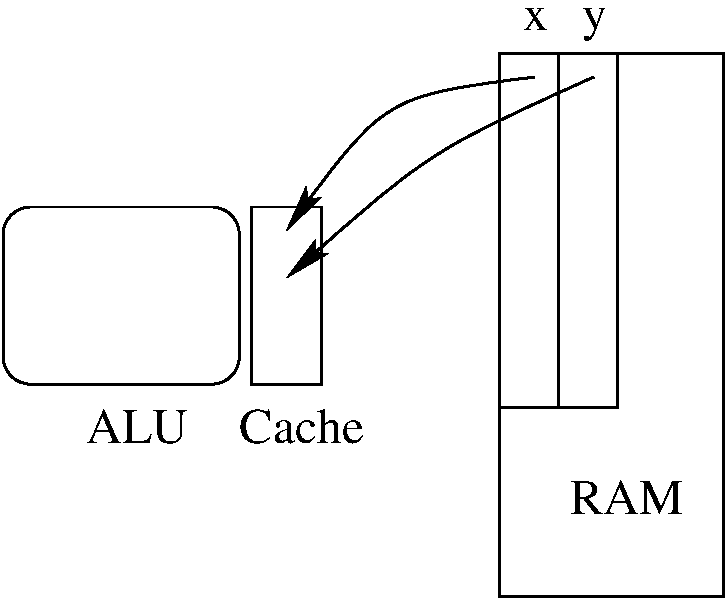
\includegraphics[width=0.4\textwidth]{kernel-fusion-1.pdf}
 \end{center}


\end{frame}



\begin{frame}[fragile]{Expression Template Limitations}

 \begin{block}{Expression Templates are Not Enough}
  \begin{itemize}
   \item Consider
    \begin{lstlisting}
 u = x + y;
 v = x - y;
    \end{lstlisting}
   \item Suboptimal performance with almost any library
  \end{itemize}
 \end{block}
 
 \begin{center}
  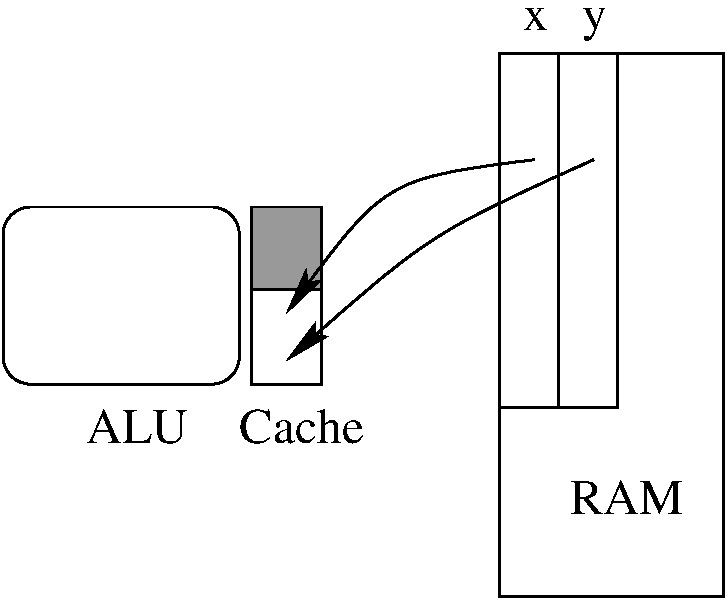
\includegraphics[width=0.4\textwidth]{kernel-fusion-2.pdf}
 \end{center}


\end{frame}


\begin{frame}[fragile]{Expression Template Limitations}

 \begin{block}{Expression Templates are Not Enough}
  \begin{itemize}
   \item Consider
    \begin{lstlisting}
 u = x + y;
 v = x - y;
    \end{lstlisting}
   \item Suboptimal performance with almost any library
  \end{itemize}
 \end{block}

 \begin{block}{OpenCL Kernel Generation}
   \begin{itemize}
    \item Separate temporary avoidance from operation execution
    \begin{lstlisting}
 viennacl::kernel_fusion(true); //API not final!
 u = x + y;
 v = x - y;
 ...
 viennacl::kernel_fusion(false);
    \end{lstlisting}
    \item Semi-transparent kernel fusion in preparation (scheduler)
   \end{itemize}
 \end{block}
\end{frame}


\begin{frame}{Expression Template Limitations}

 \begin{block}{Benchmark Results}
  \begin{center}
   $\beta \leftarrow x^T \cdot (2x + y)$ \\
   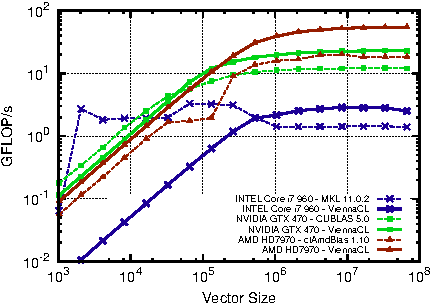
\includegraphics[width=0.75\textwidth]{figures/daxpy_ddot.pdf} \\
  \end{center}
   \scriptsize Tillet \textit{et al.}, HotPar '13

 \end{block}

\end{frame}
